\documentclass[12pt,a4paper]{scrartcl}

\usepackage[utf8]{inputenc}
\usepackage[T1]{fontenc}

\usepackage[french]{babel,varioref}

\usepackage{multicol}
\usepackage{subfig}

\usepackage{enumitem}

\usepackage{color}
\usepackage{hyperref}
\hypersetup{
    colorlinks,
    citecolor=black,
    filecolor=black,
    linkcolor=black,
    urlcolor=black
}

\usepackage{amsthm}

\usepackage[most]{tcolorbox}
\tcbuselibrary{listingsutf8}

\usepackage{ifplatform}

\usepackage{xstring}

\usepackage{fancyvrb}


% MISC

\tcbset{%
	sharp corners,%
	left=1mm, right=1mm,%
	bottom=1mm, top=1mm,%
	colupper=red!75!blue%
}

\newcommand\examplestarted{%%
    \par\smallskip
    \begingroup%%
        \centering%%
        \setlength{\fboxrule}{0.7pt}%%
        \rule[0.4ex]{5em}{0.7pt}%%
        \framebox{\small\vphantom{pE}Mise en forme - Début}%%
        \rule[0.4ex]{5em}{0.7pt}%%
        \par\smallskip
    \endgroup%%
}

\newcommand\examplefinished{%%
    \par\smallskip
    \begingroup%%
        \centering%%
        \setlength{\fboxrule}{0.7pt}%%
        \rule[0.4ex]{5.5em}{0.7pt}%%
        \framebox{\small\vphantom{pE}Mise en forme - Fin}%%
        \rule[0.4ex]{5.5em}{0.7pt}%%
        \par\smallskip
    \endgroup%%
}

\setlength{\parindent}{0cm}

\theoremstyle{definition}
\newtheorem*{remark*}{Remarque}
\newtheorem{remark}{Remarque}

\usepackage[raggedright]{titlesec}

\titleformat{\paragraph}[hang]{\normalfont\normalsize\bfseries}{\theparagraph}{1em}{}
\titlespacing*{\paragraph}{0pt}{3.25ex plus 1ex minus .2ex}{0.5em}


\makeatletter
    \newcommand\resetallcnt{
    	\setcounter{lyxam@counter@topic}{0}
    	\setcounter{lyxam@counter@exercise}{0}
    	\setcounter{lyxam@counter@problem}{0}
    	\setcounter{lyxam@counter@bonus}{0}
    	\setcounter{lyxam@counter@subpart}{0}
    }
\makeatother


% Technical IDs

\newwrite\tempfile
\immediate\openout\tempfile=x-\jobname.macros-x.txt
\AtEndDocument{\immediate\closeout\tempfile}


\newcommand\IDconstant[1]{%
    \immediate\write\tempfile{constant@#1}%
}


\makeatletter
\newcommand\IDmacro{\@ifstar{\@IDmacroStar}{\@IDmacroNoStar}}

\newcommand\@IDmacroNoStar[3]{%
    \texttt{%
    	\textbackslash#1%
    	\IfStrEq{#2}{0}{}{%
    		\,\,[#2 Option%
			\IfStrEq{#2}{1}{}{s}]%
		}%
	    \IfStrEq{#3}{}{}{%
    		\,\,(#3 Argument%
			\IfStrEq{#3}{1}{}{s})%
		}
   	}
    \immediate\write\tempfile{macro@#1@#2@#3}%
}

\newcommand\@IDmacroStar[2]{%
    \@IDmacroNoStar{#1}{0}{#2}%
}


\newcommand\IDenv{\@ifstar{\@IDenvStar}{\@IDenvNoStar}}

\newcommand\@IDenvNoStar[3]{%
    \texttt{%
    	\textbackslash#1%
    	\IfStrEq{#2}{0}{}{%
    		\,\,[#2 Option%
			\IfStrEq{#2}{1}{}{s}]%
		}%
	    \IfStrEq{#3}{}{}{%
    		\,\,(#3 Argument%
			\IfStrEq{#3}{1}{}{s})%
		}
   	}
    \immediate\write\tempfile{env@#1@#2@#3}%
}

\newcommand\@IDenvStar[2]{%
    \@IDenvNoStar{#1}{0}{#2}%
}


\newcommand\@IDoptarg{\@ifstar{\@IDoptargStar}{\@IDoptargNoStar}}

\newcommand\@IDoptargStar[2]{%
	\vspace{0.5em}
	--- \texttt{#1%
		\IfStrEq{#2}{}{:}{\,#2:}%
	}%
}

\newcommand\@IDoptargNoStar[2]{%
	\IfStrEq{#2}{}{%
		\@IDoptargStar{#1}{}%
	}{%
		\@IDoptargStar{#1}{\##2}%
	}%
}


\newcommand\IDkey[1]{%
	\@IDoptarg*{Option}{{\itshape "#1"}}%
}


\newcommand\IDoption[1]{%
	\@IDoptarg{Option}{#1}%
}


\newcommand\IDarg[1]{%
	\@IDoptarg{Argument}{#1}%
}
\makeatother

\usepackage[fr]{lyxam}


\begin{document}

\renewcommand\labelitemi{\raisebox{0.125em}{\tiny\textbullet}}
\renewcommand{\labelitemii}{---}

\title{%
	Le package \texttt{lyxam}:\\%
	des mises en forme clés en main\\%
	pour des fiches d'exercices\\%
	{\footnotesize Code source disponible sur \url{https://github.com/bc-latex/ly-xam}.}\\%
	{\footnotesize Version \texttt{1.0.0-beta} développée et testée sur \macosxname{}.}%
}
\author{Christophe BAL}
\date{2017-12-13}

\maketitle


\vspace{2em}

\hrule

\tableofcontents

\vspace{1.5em}

\hrule

\newpage



\section{Introduction}

Le but du tout petit package \verb+lyxam+ est de fournir un moyen simple de rédiger des feuilles d'exercices pour des entraînements ou des évaluations dans le cadre d'un enseignement.




\section{Les options du package}

Avant d'entrer dans le vif du sujet, nous donnons ici toutes les options utilisables lors de l'appel du package via \verb+\usepackage[...]{lyxam}+.

\begin{itemize}
	\item \verb+en+, valeur par défaut
	\footnote{
		Sorry for the french frogs that we are... (Trad. : Désolé pour les grenouilles françaises que nous sommes...)
	}, et \verb+fr+ permettent d'indiquer d'utiliser l'anglais ou le français pour tous les textes ajoutés par \verb+lyxam+.

	\item \verb+nohf+ permet de ne pas afficher les en-têtes et les pieds de page.
	Les lettres \verb+hf+ sont pour "\textbf{h}-eaders" et "\textbf{f}-ooters", soit "en-tête" et "pied de page" en français.

	\item \verb+nopts+ cache les points indiquant le note total pour un devoir et un barème grossier pour chaque exercice.

	\item \verb+short+ demande d'utiliser si possible des noms abrégés pour les types d'exercices, les points et le temps.

	\item \verb+nosrc+ empêchera l'affichage des sources utilisées.

	\item \verb+noabout+ ne tient pas compte des informations complémentaires données pour les thèmes, les exercices et les parties.

	\item Pour finir, voici les différents styles de mise en forme disponibles (dans le dossier \verb+examples+ se trouvent divers \verb+PDFs+ donnant un aperçu de ces styles prédéfinis).
	\begin{itemize}[label={\small\textbullet}]
        \item Style par défaut, \verb+mini+ propose une mise forme minimaliste utilisant le moins de fioritures possibles.
        
        \item \verb+apmep+ est inspiré fortement de la mise en forme des sujets de BAC que l'on trouvait en 2017 sur le site \href{https://www.apmep.fr}{APMEP} (Association des Professeurs de Mathématiques de l'Enseignement Public).
        
        \item \verb+book+ fournit une mise forme utile dans un livre ou un cours. Attention car cette option ne crée pas d'en-têtes, pas de pieds de page, et elle ne mettra pas en forme de capsules pour le nom et le prénom des élèves même si cela est demandé.
        
        \item \verb+ecolo+ mélange les styles \verb+mini+ et \verb+book+ pour produire des devoirs très peu consommateur d'espaces.
        
        \item \verb+linebox+ utilise des lignes et des cadres (il a été conçu à l'origine pour les corrigés de l'auteur de \verb+lyxam+).
    \end{itemize}
\end{itemize}


\begin{remark*}
	Dans la suite de cette documentation nous invoquons juste l'option \verb+fr+.
	Autrement dit, nous passons par \verb+\usepackage[fr]{lyxam}+ donc ce sera le style par défaut \verb+mini+ qui donnera la mise en forme.
\end{remark*}




\section{Quel devoir donnez-vous ?}

    \subsection{La commande \texttt{\textbackslash exam}}

La commande \verb+\exam+ permet de donner des informations générales à propos du devoir.
Le code ci-dessous utilise toutes les options disponibles, et la figure \ref{style:default} \vpageref{style:default} donne un aperçu du rendu obtenu dans ce cas.

\begin{tcblisting}{listing only}
\exam[deliver  = short,%
      kind     = D.S.,%
      nb       = 1,%
      subnb    = Sujet A,%
      subject  = Mathématiques,%
      theme    = Probabilités,%
      sector   = Série Scientifique,%
      class    = 1S4,%
      location = Lycée MONGE (Chambéry),%
      date     = 20/10/2017,%
      time     = 2h,%
      pts      = 20]
\end{tcblisting}


\begin{figure}[!tbp]
  \setlength{\fboxrule}{1.5pt}
  \centering
  \fbox{
\includegraphics[width=0.43\linewidth]{example-doc[fr]-0.jpg}}
  \hfill
  \fbox{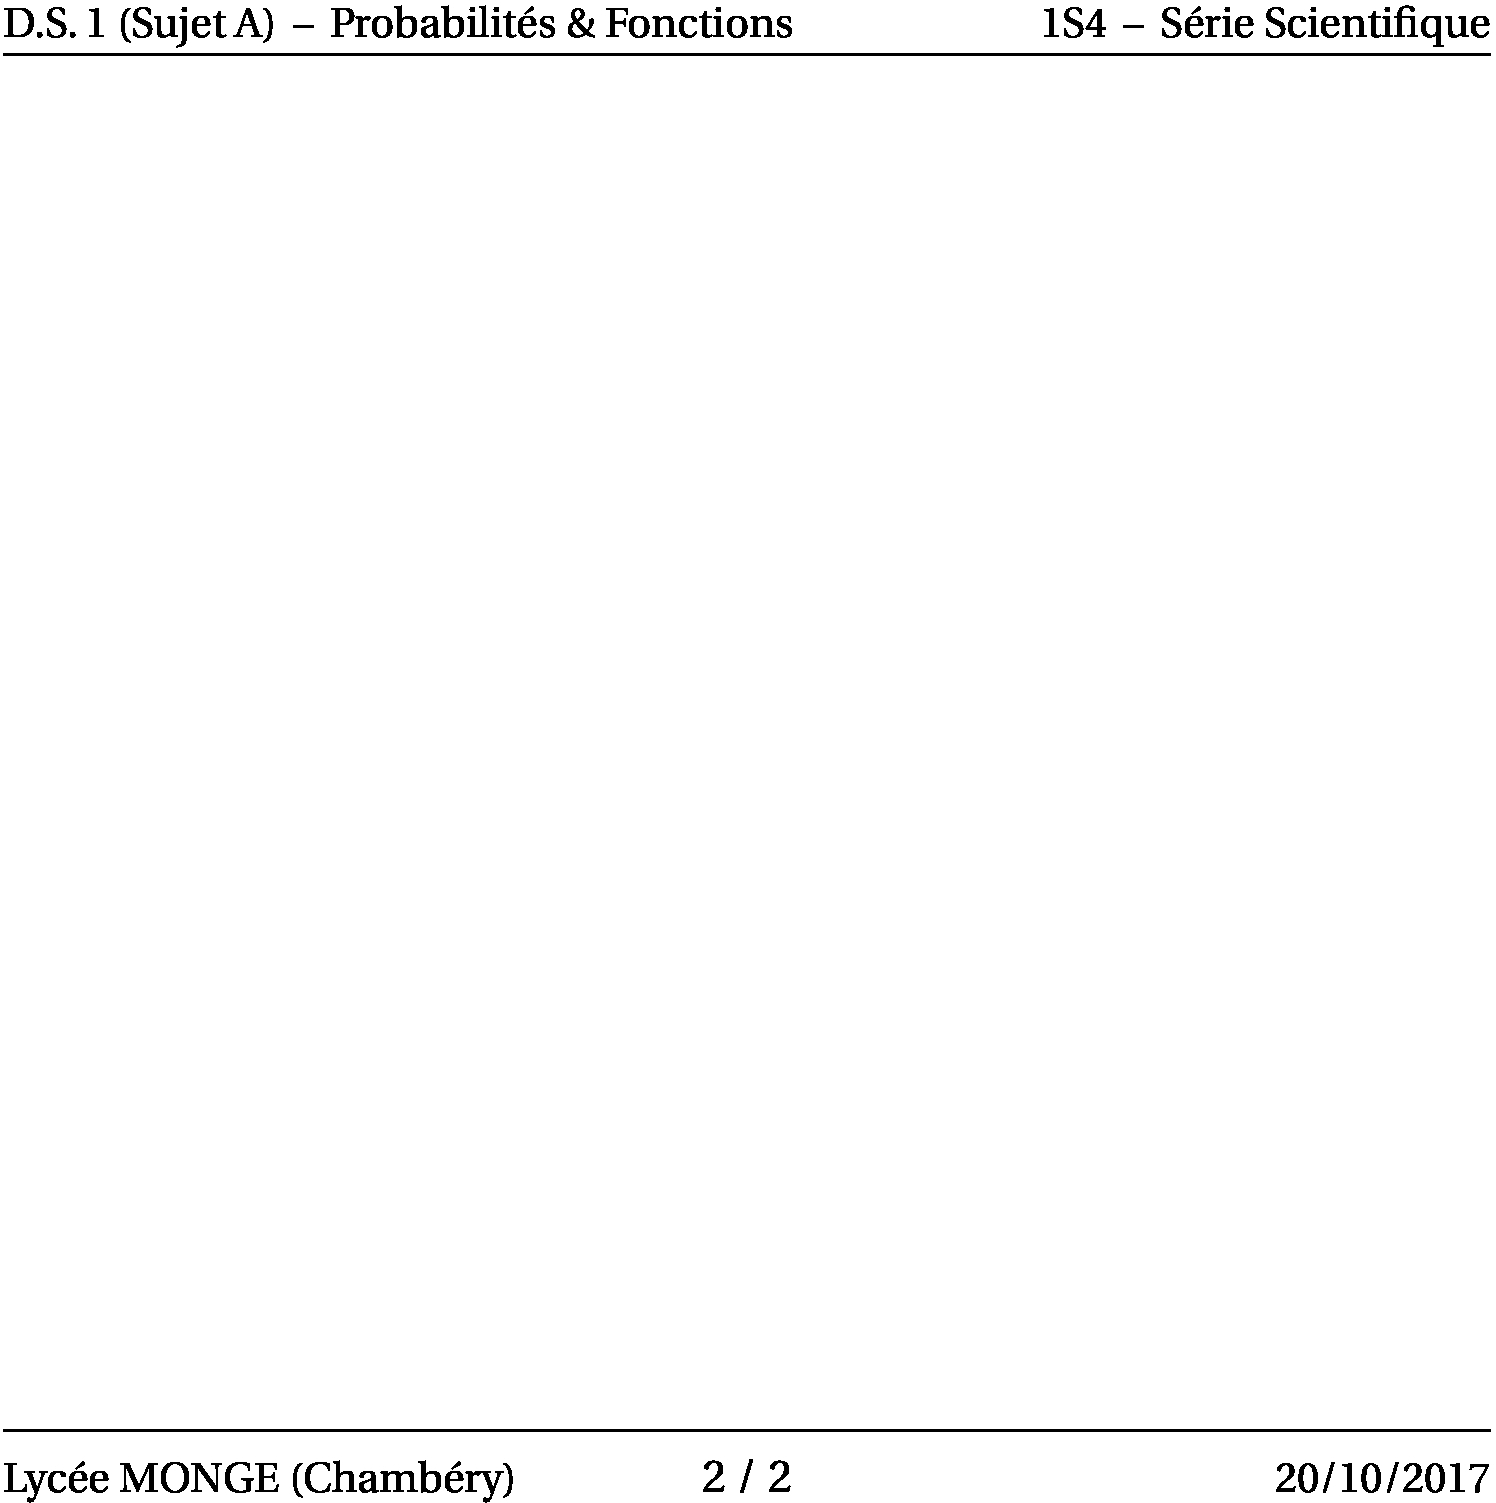
\includegraphics[width=0.43\linewidth]{example-doc[fr]-1.jpg}}
  \caption{Style par défaut.}
  \label{style:default}
\end{figure}

Présentons maintenant en détail chacun des paramètres qui sont tous optionnels. Lorsqu'aucune valeur par défaut n'est indiquée, c'est que cette valeur est un texte vide.

\begin{enumerate}
    \item \verb+deliver+, valant \verb+no+ par défaut, est pour un sujet à rendre avec la copie.
    \begin{itemize}
        \setlength\itemsep{0em}

        \item On peut indiquer \verb+deliver = short+ où \emph{"short"} signifie \emph{"court"}. Ceci affichera une "petite" capsule où l'étudiant renseignera son prénom et son nom. Idéal pour le format \verb+A4+.

        \item Avec \verb+deliver = long+, la capsule sera plus grande. Idéal pour le format \verb+A5+.

        \item Ne pas utiliser l'option revient à passer par \verb+deliver = no+.
    \end{itemize}

    \item \verb+kind+, valant \verb+Test+ par défaut, est le type de devoir : un \emph{"D.S."}, un \emph{"D.M."}, une \emph{"Interrogation Surprise"}, une \emph{"Fiche d'entraînement"}, une \emph{"Activité"}...
    Vous noterez que le terme \emph{"devoir"} ne se limite pas juste aux devoirs notés.

    \item \verb+nb+ est le numéro du devoir.

    \item \verb+subnb+ permet d'indiquer une sorte de numérotation secondaire. C'est utile par exemple pour indiquer \emph{"Sujet A"}, \emph{"Sujet B"} ...

    \item \verb+subject+ permet de donner la thématique générale du devoir comme par exemple \emph{"Mathématiques"}, \emph{"Informatique Générale"}...

    \item \verb+theme+ complète la thématique générale en indiquant un ou des points particuliers comme par exemple \emph{"Probabilités"}, \emph{"Réseaux"} ...

    \item \verb+sector+ sert à indiquer une section, au sens administratif, à laquelle s'adresse le devoir. Par exemple, pour un sujet de Baccalauréat S en France, on serait amené à utiliser \verb+sector = Série Scientifique+.

    \item \verb+class+ indique la classe et/ou le groupe auquel est destiné le devoir.

    \item \verb+location+ vous permet d'indiquer un lieu géographique, typiquement un établissement scolaire ou universitaire.

    \item \verb+date+ est pour la date du devoir.

    \item \verb+time+ est pour la durée du devoir.

    \item \verb+pts+ permet d'indiquer sur combien de points sera évalué un devoir.
\end{enumerate}


    \subsection{Fiche technique}

\IDmacro{exam}{12}{}

\IDkey{kind} le type de devoir, la valeur par défaut étant \verb+Test+.

\IDkey{deliver} pour un sujet à rendre, ou non, avec une zone pour le nom et le prénom de l'étudiant. Trois valeurs possibles : \verb+no+, valeur par défaut, \verb+long+ et \verb+short+.

\IDkey{nb} le numéro du devoir.

\IDkey{subnb} une numérotation secondaire du devoir.

\IDkey{subject} la matière, le sujet au sens large du devoir.

\IDkey{theme} un sous-thème ou une sous-partie de la matière ou du sujet du devoir.

\IDkey{sector} un secteur, une section, au sens administratif, à laquelle s'adresse le devoir.

\IDkey{class} la classe concernée par le devoir.

\IDkey{location} le lieu géographique où a lieu le devoir.

\IDkey{date} le texte donnant la date du devoir.

\IDkey{time} le texte indiquant juste la durée du devoir.

\IDkey{pts} le nombre total de points pour évaluer un devoir.




\newcommand\exosoptionsdescription{
Toutes les options données ci-dessous sont facultatives. Attention car avec les versions simplement étoilées il faut utiliser \texttt{id},
tandis qu'avec les versions doublement étoilées on doit se servir de l'option \texttt{title}.
}

\newcommand\exosoptions{
\IDkey{pts} le nombre de points avec le cas particulier de $0$ qui demande d'afficher "Non noté".

\IDkey{time} la durée de l'exercice.

\IDkey{id} un texte de votre choix pour remplacer le numéro (ceci a pour effet de bloquer temporairement la numérotation).

\IDkey{title} un titre.

\IDkey{about} une petite indication liée à l'exercice (comme par exemple qu'il ne s'adresse qu'aux élèves motivés).

\IDkey{src} la source utilisée pour confectionner l'exercice.
}


\section{Les exercices}

    \subsection{Important pour la suite}

Rappelons que tous les exemples utilisés dans cette documentation ont été obtenus en utilisant \verb+\usepackage[fr]{lyxam}+ dans le préambule ce qui charge le style par défaut parmi les différents styles proposés (voir le dossier \verb+examples+ pour choisir un style prédéfini).


    \subsection{Différents types d'exercices}

Voici l'ensemble des commandes disponibles pour indiquer un type d'exercice.

% All kind of level 2 contexts - START
\begin{itemize}
\makeatletter
    \item \verb+\activity+ correspond à "\lyxam@text@activity{}".
    
    \item \verb+\bonus+ correspond à "\lyxam@text@bonus{}".
    
    \item \verb+\exercise+ correspond à "\lyxam@text@exercise{}".
    
    \item \verb+\mcq+ correspond à "\lyxam@text@mcq{}".
    
    \item \verb+\praticalwork+ correspond à "\lyxam@text@praticalwork{}".
    
    \item \verb+\problem+ correspond à "\lyxam@text@problem{}".
\makeatother
\end{itemize}
% All kind of level 2 contexts - END

Dans la suite, nous donnerons des exemples principalement avec la commande \verb+\exercise+. Ceci n'est pas gênant car le principe reste identique pour les autres commandes.


    \subsection{Numérotation minimaliste}

En \textbf{compilant deux fois} au moins, \verb+lyxam+ va pouvoir donner une numérotation minimaliste de vos exercices.
Par exemple, ci-dessous on obtient classiquement des exercices tous numérotés (vous noterez que les problèmes et les bonus ont leur propre numérotation).
Que souhaite-t-on avoir dans un sujet ne contenant qu'un seul problème et un seul bonus ? Nul besoin ici d'avoir un numéro pour ces derniers. C'est ce que fait \verb+lyxam+.

\resetallcnt{}

\begin{tcblisting}{listing only}
\exercise
\exercise
\problem
\bonus
\end{tcblisting}
\examplestarted    % ----- START ----- %
\exercise
\exercise
\problem
\bonus
\examplefinished   % -----  END  ----- %



    \subsection{Indiquer les points attribués à un exercice}

L'option \verb+pts+ permet de donner sommairement le nombre total de points attribués à un exercice, ou bien d'indiquer qu'un exercice n'est pas noté. Voici comment faire.

\resetallcnt{}

\begin{tcblisting}{listing only}
\exercise[pts = 5]
Bla, bla, bla, bla, bla, ...

\exercise[pts = 0]
Bla, bla, bla, bla, bla, ...
\end{tcblisting}
\examplestarted    % ----- START ----- %
\exercise[pts = 5]
Bla, bla, bla, bla, bla, ...

\exercise[pts = 0]
Bla, bla, bla, bla, bla, ...
\examplefinished   % -----  END  ----- %

\begin{remark*}
La section \ref{exercises:score} explique comment indiquer un barème assez détaillé tout en obtenant un fichier externe pour faciliter la correction de devoirs d'étudiant.
\end{remark*} 



    \subsection{Utiliser une numérotation "maison"}

La version étoilée \verb+\exercise*+ permet d'afficher un texte de son choix à la place de la numérotation automatique (dans ce cas, la numérotation automatique est mise en attente). Voici un exemple concret d'utilisation.

\begin{tcblisting}{listing only}
\exercise*[id = facultatif]
Bla, bla, bla, bla, bla, ...
\end{tcblisting}
\examplestarted    % ----- START ----- %
\exercise*[id = facultatif]
Bla, bla, bla, bla, bla, ...
\examplefinished   % -----  END  ----- %



    \subsection{Cacher le texte "Exercice"}

La version doublement étoilée \verb+\exercise**+ permet de cacher le contexte qui du point de vue de \verb+lyxam+ est le texte indiquant le type d'exercice (ceci est très pratique pour les sous-parties présentées dans la section \ref{exercises:subparts}). Dans ce genre de situation, il faut obligatoirement donner un titre.

\begin{tcblisting}{listing only}
\exercise**[title = Juste mon titre]
Bla, bla, bla, bla, bla, ...
\end{tcblisting}
\examplestarted    % ----- START ----- %
\exercise**[title = Juste mon titre]
Bla, bla, bla, bla, bla, ...
\examplefinished   % -----  END  ----- %


    \subsection{Toutes les options en action}

Les fiches techniques données dans la section \ref{exercises:technicalids} expliquent le champs d'utilisation de chaque option.

\begin{tcblisting}{listing only}
\exercise*[pts   = 0,
           time  = 3 jours,
           id    = facultatif,
           title = Devinette,
           about = Pour spécialiste uniquement,
           src   = Le livre des experts]
Bla, bla, bla, bla, bla, ...
\end{tcblisting}
\examplestarted    % ----- START ----- %
\exercise*[pts   = 0,
           time  = 3 jours,
           id    = facultatif,
           title = Devinette,
           about = Pour spécialiste uniquement,
           src   = Le livre des experts]
Bla, bla, bla, bla, bla, ...
\examplefinished   % -----  END  ----- %


    \subsection{Fiches techniques} \label{exercises:technicalids}

\exosoptionsdescription{}

\begin{multicols}{2}% IDmacro - All kind of level 2 contexts - START
\IDmacro{activity}{6}{}

\IDmacro{activity*}{6}{}

\IDmacro{activity**}{6}{}

\vspace{0.7ex}
\IDmacro{bonus}{6}{}

\IDmacro{bonus*}{6}{}

\IDmacro{bonus**}{6}{}

\vspace{0.7ex}
\IDmacro{exercise}{6}{}

\IDmacro{exercise*}{6}{}

\IDmacro{exercise**}{6}{}

\vspace{0.7ex}
\IDmacro{mcq}{6}{}

\IDmacro{mcq*}{6}{}

\IDmacro{mcq**}{6}{}

\vspace{0.7ex}
\IDmacro{praticalwork}{6}{}

\IDmacro{praticalwork*}{6}{}

\IDmacro{praticalwork**}{6}{}

\vspace{0.7ex}
\IDmacro{problem}{6}{}

\IDmacro{problem*}{6}{}

\IDmacro{problem**}{6}{}

% IDmacro - All kind of level 2 contexts - END
\end{multicols}

\vspace{-1em}

\exosoptions{}



\section{Indiquer des sous-parties dans vos exercices} \label{exercises:subparts}

    \subsection{Un exemple suffit\dots{} ou presque}

La commande \verb+\subpart+, avec les mêmes options que les commandes de type \verb+\exercice+, sert pour des sous-parties d'un exercice qui seront numérotées relativement aux exercices comme le montre l'exemple suivant.

\resetallcnt{}

\begin{tcblisting}{listing only}
\exercise
\subpart
\subpart

\exercise
\subpart
\subpart
\end{tcblisting}
\examplestarted    % ----- START ----- %
\exercise
\subpart
\subpart

\exercise
\subpart
\subpart
\examplefinished   % -----  END  ----- %


    \subsection{Fiche technique}

\exosoptionsdescription{}

\bigskip

% IDmacro - All kind of level 3 contexts - START
\IDmacro{subpart}{6}{}

\IDmacro{subpart*}{6}{}

\IDmacro{subpart**}{6}{}

% IDmacro - All kind of level 3 contexts - END

\exosoptions{}



\section{Regrouper vos exercices par thèmes}

    \subsection{Un exemple suffit\dots{} ou presque}

La commande \verb+\topic+, avec les mêmes options que les commandes de type \verb+\exercice+, sert juste à regrouper des exercices par thématiques : fût un temps où dans les brevets du collège, il y avait une partie numérique et une autre géométrique.
Chaque nouvelle utilisation de \verb+\topic+ remet juste à zéro la numérotation des sous-parties mais pas celles des contextes de type \verb+\exercice+.

\resetallcnt{}

\begin{tcblisting}{listing only}
\topic
\exercise
\exercise

\topic
\exercise
\end{tcblisting}
\examplestarted    % ----- START ----- %
\topic
\exercise
\exercise

\topic
\exercise
\examplefinished   % -----  END  ----- %


    \subsection{Fiche technique}

\exosoptionsdescription{}

\bigskip

% IDmacro - All kind of level 1 contexts - START
\IDmacro{topic}{6}{}

\IDmacro{topic*}{6}{}

\IDmacro{topic**}{6}{}

% IDmacro - All kind of level 1 contexts - END

\exosoptions{}



\section{Personnaliser les numérotations}

    \subsection{Un petit exemple}

En mettant un peu les mains dans le cambouis, on peut modifier à sa guise la numérotation de chaque type d'exercice. Voici un exemple tapé directement dans un fichier \verb+tex+, ce qui impose d'employer \verb+\makeatletter...\makeatother+.

\resetallcnt{}

\begin{tcblisting}{listing only}
\makeatletter
    \renewcommand\lyxam@counter@exercise@style[1]{-- \arabic{#1} --}
\makeatother

\exercise
\exercise
\end{tcblisting}
\examplestarted    % ----- START ----- %
\makeatletter
    \renewcommand\lyxam@counter@exercise@style[1]{-- \arabic{#1} --}
\makeatother

\exercise
\exercise
\examplefinished   % -----  END  ----- %


    \subsection{Fiches techniques}

% IDmacro - All styles for counters - START
\IDmacro{lyxam@counter@activity@style}{0}{1}

\IDmacro{lyxam@counter@bonus@style}{0}{1}

\IDmacro{lyxam@counter@exercise@style}{0}{1}

\IDmacro{lyxam@counter@mcq@style}{0}{1}

\IDmacro{lyxam@counter@praticalwork@style}{0}{1}

\IDmacro{lyxam@counter@problem@style}{0}{1}

\IDmacro{lyxam@counter@subpart@style}{0}{1}

\IDmacro{lyxam@counter@topic@style}{0}{1}
% IDmacro - All styles for counters - END

\IDarg{} the \LaTeX{} counter associated to the context.





\section{Utiliser un préambule}

    \subsection{Un exemple avec toutes les options}

L'environnement \verb+\preamble+ sert à rédiger un ou plusieurs paragraphes en préambule de tout un examen, d'un thème, d'un exercice ou d'une partie.
Il propose deux options : l'une \verb+center+ pour centrer le contenu à l'intérieur du préambule, l'autre \verb+scale+ pour indiquer un coefficient multiplicatif pour la largeur allouée au préambule (ce coefficient est multiplié à \verb+\linewidth+ pour calculer la largeur souhaitée).

\resetallcnt{}

\begin{tcblisting}{listing only}
\begin{preamble}[scale = 0.75, center]
    Cet exercice est indépendant \verb+;-)+. Bla, bla, bla, bla, bla, bla,
    bla, bla, bla, bla, bla, bla, bla, bla, bla, bla, bla, bla, bla\dots
\end{preamble}

\exercise
\begin{preamble}
    Dans cet exercice, tout trace de recherche sera prise en compte à
    condition de ne pas explorer le Pôle Nord quand on s'intéresse
    au Pôle Sud. Quoique\dots
\end{preamble}

Tenter, chercher, trouver\dots
\end{tcblisting}
\examplestarted    % ----- START ----- %
\begin{preamble}[scale = 0.75, center]
    Cet exercice est indépendant \verb+;-)+. Bla, bla, bla, bla, bla, bla,
    bla, bla, bla, bla, bla, bla, bla, bla, bla, bla, bla, bla, bla\dots
\end{preamble}

\exercise
\begin{preamble}
    Dans cet exercice, tout trace de recherche sera prise en compte à
    condition de ne pas explorer le Pôle Nord quand on s'intéresse
    au Pôle Sud. Quoique\dots
\end{preamble}

Tenter, chercher, trouver\dots
\examplefinished   % -----  END  ----- %


    \subsection{Fiches techniques}

\IDenv{preamble}{2}{}

\IDkey{scale} un nombre, valant $1$ par défaut, qui sera multiplié à la largeur d'une ligne pour obtenir la largeur souhaitée pour le préambule.

\IDkey{center} un booléen, valant \verb+false+ par défaut, pour centrer ou non le contenu du préambule (notez que \verb+center+ est un raccourci de \verb+center = true+).





\section{Détailler le barème} \label{exercises:score}

score : affiche + crée fichier externe

nopts + score : cahce mais crée fichier externe



\section{Historique}

Tous les changements sont décrits en anglais uniquement dans le dossier \verb+change_log+ : voir le code source de \verb+lyxam+ sur \verb+github+. Nous ne donnons ici qu'un très bref historique de \verb+lyxam+.

\medskip

\begin{description}[leftmargin=1em]
    \setlength\itemsep{1em}
    \item[2017-12-13] Nouvelle version majeure \verb+1.0.0-beta+.
        \begin{itemize}
            \item La grosse nouveauté est la possibilité d'indiquer un barème détaillé via l'option de package \verb+score+ et la macro \verb+\scpts+.

            \item Les exercices ont dorénavant une version étoilée qui cache le numéro et demande d'utiliser \verb+id+, et une version doublement étoilée qui cache le type d'exercice et nécessite l'emploi de \verb+title+.

            \item Une nouvelle option \verb+pts+ pour la macro \verb+\exam+ permet d'indiquer sur combien un devoir sera évalué.

            \item Les options de package \verb+about+, \verb+hf+, \verb+noshort+, \verb+pts+ et \verb+src+ ont été supprimées car elles étaient inutiles.
        \end{itemize}


    \item[2017-12-02] Nouvelle version mineure \verb+0.3.0-beta+.
    \begin{itemize}
        \item L'option de package \verb+mini+ fournit un style de mise en forme minimaliste. Ce sera le style par défaut.

        \item L'option de package \verb+book+ a été ajouté pour insérer des exercices dans un document de type cours ou livre.

        \item L'option de package \verb+ecolo+ mélange les mises en forme de \verb+mini+ et \verb+book+ pour rédiger des devoirs en gaspillant le moins d'espaces possible.
    \end{itemize}


    \item[2017-11-28] Nouvelle version mineure \verb+0.2.0-beta+.
    \begin{itemize}
        \item L'option de package \verb+linebox+ fournit un nouveau style de mise en forme.

        \item Les options de package \verb+short+ et \verb+noshort+ permettent d'indiquer ou non en abrégé, si possible, les types d'exercices, les points et le temps.

        \item Les options de package \verb+about+, valeur par défaut, et \verb+noabout+ feront afficher ou non les informations complémentaires sur les thèmes, les exercices et les parties.

        \item L'option \verb+render+ de la macro \verb+\exam+ a été renommée \verb+deliver+ (ce qui semble plus correct).

        \item Ajout de deux options à l'environnement \verb+\preamble+ : l'une pour centrer ou non le contenu, et l'autre pour choisir la largeur occupée par le préambule.

        \item Il est maintenant possible de personnaliser la numérotation des exercices.
    \end{itemize}


    \item[2017-11-12] Nouvelle version mineure \verb+0.1.0-beta+.
    \begin{itemize}
        \item Les nouvelles options \verb+hf+ et \verb+nohf+ permettent au chargement du package de montrer ou cacher les en-têtes et les pieds de page.

        \item L'option \verb+preamble+ de la macro \verb+\exam+ disparait pour laisser place au nouvel environnement \verb+\begin{preamble}...\end{preamble}+ utilisable n'importe où.

        \item Pour la macro \verb+\exam+, tous les paramètres sont optionnels.

        \item Pour les macros du type \verb+\exercise+, le paramètre \verb+note+ a été renommé \verb+about+.

        \item En interne, l'utilisation de \verb+simplekv+ a permis une refonte complète du code en simplifiant la méthode à utiliser pour créer de nouvelles mises en page "maison".
    \end{itemize}


    \item[2017-11-03] Première version publique \verb+0.0.0-beta+.
\end{description}



\end{document}
